
%(BEGIN_QUESTION)
% Copyright 2006, Tony R. Kuphaldt, released under the Creative Commons Attribution License (v 1.0)
% This means you may do almost anything with this work of mine, so long as you give me proper credit

A filled-system temperature indicator is calibrated in the instrument shop with the sensing bulb at the same level (height) as the bourdon tube indicating element.  In the field, however, the sensing bulb is significantly elevated from the bourdon tube's height.

$$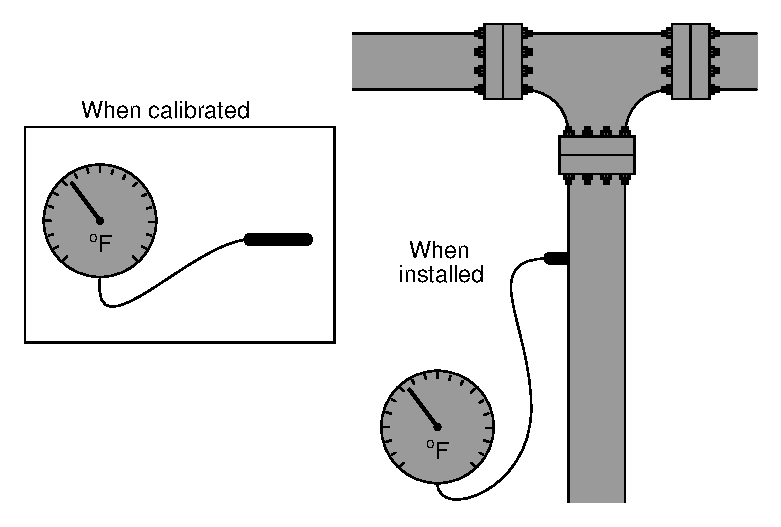
\includegraphics[width=15.5cm]{i00360x01.eps}$$

Will this cause a measurement error?  If so, what type of error (zero or span shift) will it be?

\vskip 20pt \vbox{\hrule \hbox{\strut \vrule{} {\bf Suggestions for Socratic discussion} \vrule} \hrule}

\begin{itemize}
\item{} Will all classes of filled-bulb temperature gauges be affected the same way by an offset in height?
\item{} Will a measurement error develop if the gauge is positioned {\it above} the sensing bulb?
\item{} How is this phenomenon similar to issues faced inferring liquid level using hydrostatic pressure?  Is there a term we use to describe it?
\end{itemize}

\underbar{file i00360}
%(END_QUESTION)





%(BEGIN_ANSWER)

Differences in elevation between the sensing bulb and the indicating element only affect some classes of filled-bulb systems, not all.  For these systems, the elevation will create a zero shift.

%(END_ANSWER)





%(BEGIN_NOTES)

Differences in elevation between the sensing bulb and the indicating element only affect filled systems containing liquid in the capillary tube.  This includes Class I, Class IIA, Class IID, and Class V filled systems.  Class III filled systems are unaffected by elevation or suppression because their working fluid is simply gas, and there is negligible hydrostatic pressure generated by that elevation or suppression of gas.

\vskip 10pt

In the example shown, the zero shift will be such that the indicator will read falsely high, due to the hydrostatic pressure generated by the elevation.

%INDEX% Measurement, temperature: filled-bulb system

%(END_NOTES)


